% TaskFlow DevSecOps CI/CD report -- Overleaf (pdfLaTeX)
% Upload this file + the figures/ folder, then Recompile.
\documentclass[11pt,a4paper]{article}

\usepackage[T1]{fontenc}
\usepackage[utf8]{inputenc}
\usepackage{lmodern}
\usepackage[margin=1.8cm]{geometry}
\usepackage{xcolor}
\usepackage{graphicx}
\usepackage{booktabs}
\usepackage{tabularx}
\usepackage{array}
\usepackage{colortbl}
\usepackage{hyperref}
\usepackage{enumitem}
\usepackage{titlesec}
\usepackage{setspace}
\usepackage{tikz}
\usepackage[most]{tcolorbox}
\usepackage{caption}
\captionsetup{
  font={small,color=muted},
  labelfont={bf,color=statblue},
  skip=6pt,
  justification=raggedright,
  singlelinecheck=false
}

\hypersetup{
  colorlinks=true,
  linkcolor=linkblue,
  urlcolor=linkblue,
  pdftitle={DevSecOps CI/CD Pipeline Report -- TaskFlow Honeypot}
}

\definecolor{pagebg}{HTML}{1B1F24}
\definecolor{cardbg}{HTML}{252A31}
\definecolor{cardbg2}{HTML}{2C323A}
\definecolor{muted}{HTML}{9AA3AE}
\definecolor{titlew}{HTML}{F3F4F6}
\definecolor{line}{HTML}{3A424C}
\definecolor{statred}{HTML}{F87171}
\definecolor{statblue}{HTML}{60A5FA}
\definecolor{statgreen}{HTML}{34D399}
\definecolor{statwhite}{HTML}{E5E7EB}
\definecolor{warnbg}{HTML}{3F3516}
\definecolor{warnfg}{HTML}{FBBF24}
\definecolor{linkblue}{HTML}{7DD3FC}
\definecolor{beforebd}{HTML}{F87171}
\definecolor{afterbd}{HTML}{34D399}
\definecolor{headerrow}{HTML}{323842}
\definecolor{crit}{HTML}{FCA5A5}
\definecolor{high}{HTML}{FCD34D}
\definecolor{med}{HTML}{93C5FD}

\pagecolor{pagebg}
\color{titlew}
\setstretch{1.12}

\titleformat{\section}{\large\bfseries\color{titlew}}{\thesection.}{0.6em}{}
\titleformat{\subsection}{\normalsize\bfseries\color{statblue}}{\thesubsection.}{0.5em}{}
\titlespacing*{\section}{0pt}{1.3em}{0.55em}
\titlespacing*{\subsection}{0pt}{0.9em}{0.35em}

\tcbset{
  common/.style={
    enhanced,
    colback=cardbg,
    colframe=line,
    boxrule=0.4pt,
    arc=3pt,
    left=8pt,right=8pt,top=8pt,bottom=8pt,
    fontupper=\color{titlew}\small
  }
}

\newcommand{\kpi}[3]{%
  \begin{tcolorbox}[common, halign=center, valign=center, height=2.55cm]
    {\fontsize{22}{24}\selectfont\bfseries\color{#1}#2}\\[4pt]
    {\scriptsize\color{muted}#3}
  \end{tcolorbox}%
}

\newcommand{\figcap}[1]{{\centering\color{muted}\small #1\par}}

\renewcommand{\arraystretch}{1.22}
\newcolumntype{Y}{>{\raggedright\arraybackslash\color{titlew}}X}
\newcolumntype{L}{>{\raggedright\arraybackslash\color{titlew}}p}

\begin{document}

{\Huge\bfseries CI/CD pipeline report}\\[6pt]
{\color{muted}TaskFlow honeypot --- before vs after, tools, risks, vulnerabilities and countermeasures.}\\[8pt]
{\small
\href{https://github.com/belgacem-balti/honeypot/actions}{Actions}\quad
\href{https://github.com/belgacem-balti/honeypot/actions/runs/42204816549}{CI run \#1}\quad
\href{https://github.com/belgacem-balti/honeypot/actions/runs/42205865589}{CI run \#2}}
\vspace{1.1em}

\noindent
\begin{minipage}[t]{0.24\textwidth}\kpi{statred}{None}{CI before this work}\end{minipage}\hfill
\begin{minipage}[t]{0.24\textwidth}\kpi{statblue}{4}{Workflows after}\end{minipage}\hfill
\begin{minipage}[t]{0.24\textwidth}\kpi{statwhite}{11}{Stages (scan to DAST)}\end{minipage}\hfill
\begin{minipage}[t]{0.24\textwidth}\kpi{statgreen}{3m 58s}{CI run \#2 duration}\end{minipage}

\vspace{0.9em}
\begin{tcolorbox}[common, colback=warnbg, colframe=warnfg, leftrule=3pt]
\color{warnfg}\textbf{Note.}\color{titlew}\
This honeypot stays intentionally vulnerable so scanners have findings.
GitHub run \#2: Security Scans passed; tests and hardened builds passed; GHCR push failed until \texttt{packages: write}.
A green scan job means the control ran and stored a report, not that the application is safe to deploy.
\end{tcolorbox}

\section{GitHub Actions outcomes (6 Nov 2026)}

\begin{tcolorbox}[common, tabularx={Y Y Y Y},
  boxrule=0.4pt]
\textbf{Run} & \textbf{Commit} & \textbf{Duration} & \textbf{Result} \\
CI \#1 & c442e1c & 24s & Fail: \texttt{npm ci} lockfile \\
Deploy \#1 & c442e1c & 5s & Fail: no Compose secrets \\
CI \#2 & 2cf3016 & 3m 58s & Scans + tests OK; GHCR push denied \\
Deploy \#2 & 2cf3016 & skipped & Correct skip after failed CI
\end{tcolorbox}

\section{Before vs after}

\noindent
\begin{minipage}[t]{0.485\textwidth}
\begin{tcolorbox}[common, colback=cardbg2, colframe=beforebd, title={\color{statred}Before --- no pipeline}, fonttitle=\bfseries]
No workflows, no tests, hardcoded Compose secrets.\\[4pt]
Root containers, no HEALTHCHECK, no SBOM.\\[4pt]
\texttt{axios 0.21.1} / \texttt{jsonwebtoken 8.5.1} unmonitored.
\end{tcolorbox}
\end{minipage}\hfill
\begin{minipage}[t]{0.485\textwidth}
\begin{tcolorbox}[common, colback=cardbg2, colframe=afterbd, title={\color{statgreen}After --- DevSecOps path}, fonttitle=\bfseries]
Gitleaks, npm audit, Trivy, Semgrep on every push.\\[4pt]
Jest + Vitest; \texttt{Dockerfile.hardened}; CycloneDX SBOM.\\[4pt]
Deploy only if CI succeeds and secrets exist.
\end{tcolorbox}
\end{minipage}

\section{Why each tool}

\begin{tcolorbox}[common, tabularx={Y Y Y}]
\textbf{Tool} & \textbf{Why} & \textbf{Impact if missing} \\
Gitleaks & Git-history secrets & Keys reach GHCR \\
npm audit & Node CVE graph & Pinned vulns ship silent \\
Trivy fs & Cheap early scan & Wait until image build \\
Semgrep & SAST in JS/React & Only deps, not \texttt{src/} \\
Jest / Vitest & API + XSS contracts & Broken auth still ships \\
Trivy image & Built layers & Clean source, dirty image \\
SBOM & Inventory & Cannot answer what shipped \\
ZAP & Runtime HTTP & Missing headers unseen
\end{tcolorbox}

\section{Pipeline architecture}

On every push to \texttt{main} or \texttt{develop}, GitHub Actions runs \textbf{Security Scans} then, only if that job is allowed to continue, \textbf{Build \& Test}.
The first job is cheap (clone, Gitleaks, npm, Trivy fs, Semgrep). The second job is expensive (Jest, Vitest, two Docker builds, Trivy image, SBOM, GHCR).
Deploy is a separate workflow: it starts only when CI \emph{succeeds}, and it skips if secrets are empty.
ZAP is a third workflow so a 10-minute DAST run does not block every commit.

\texttt{security-scan} $\rightarrow$ \texttt{build-and-test} $\rightarrow$ (optional) \texttt{deploy} \quad;\quad weekly \texttt{security.yml} (Trivy SARIF + ZAP).

\section{Vulnerabilities and countermeasures}

The application is a honeypot: insecure files (\texttt{Dockerfile.insecure}, \texttt{docker-compose.insecure.yml}, \texttt{vulnerable.js}) remain as teaching targets. The pipeline \emph{detects} them. The hardened path (\texttt{Dockerfile.hardened}, env substitution, nginx headers) is the \emph{countermeasure} used for builds and deploy.

\subsection{Secrets}

\begin{tcolorbox}[common, tabularx={Y Y c Y}]
\textbf{Vulnerability} & \textbf{Where} & \textbf{Sev.} & \textbf{Countermeasure} \\
Hardcoded DB URL / JWT / AWS keys & \texttt{secrets.js}, \texttt{.env.production} & C & Gitleaks; gitignore \texttt{.env}; Compose \texttt{\$\{VAR\}} \\
Secrets in Docker ENV & \texttt{Dockerfile.insecure} & C & Multi-stage hardened image; no \texttt{ENV} secrets \\
Plain Kubernetes secrets & \texttt{kubernetes-secrets.yaml} & C & External secrets / Sealed Secrets (documented) \\
DB dump with keys & \texttt{backup.sql} & C & Remove from git; Gitleaks allowlist only for fixtures
\end{tcolorbox}

\subsection{Vulnerable dependencies}

\begin{tcolorbox}[common, tabularx={Y Y Y Y}]
\textbf{Package} & \textbf{Issue} & \textbf{Detector} & \textbf{Countermeasure} \\
axios 0.21.1 & CVE-2021-3749 ReDoS & npm audit, Trivy & Upgrade $\ge$ 1.6.3 in a real product \\
jsonwebtoken 8.5.1 & CVE-2022-23529 & npm audit, Trivy & Upgrade jwt; rotate \texttt{JWT\_SECRET} \\
lodash 4.17.15/19 & Prototype pollution & npm audit & Upgrade lodash \\
minimist 1.2.5 & CVE-2021-44906 & npm audit & Upgrade minimist \\
node-serialize 0.0.4 & RCE via deserialize & npm audit, Semgrep & Remove package; never \texttt{eval} user input \\
js-yaml 3.13.0 & DoS CVE-2019-6286 & npm audit & Upgrade js-yaml \\
serialize-javascript 3.1.0 & XSS CVE-2020-7660 & npm audit & Upgrade (client)
\end{tcolorbox}

\textit{Honeypot policy:} versions stay pinned so scanners keep reporting. Production policy: fail CI on HIGH/CRITICAL (\texttt{exit-code: 1}).

\subsection{Insecure code}

\begin{tcolorbox}[common, tabularx={Y Y c Y}]
\textbf{Vulnerability} & \textbf{Endpoint / function} & \textbf{Sev.} & \textbf{Countermeasure} \\
Command injection & \texttt{POST /api/vulnerable/ping} & C & Semgrep; never \texttt{exec} user input \\
Path traversal & \texttt{GET /api/vulnerable/file} & C & Canonicalize path; allowlist \\
SQL injection & \texttt{GET /api/vulnerable/user} & C & Prisma parameterized queries only \\
Insecure deserialise / eval & \texttt{POST .../deserialize} & C & Ban \texttt{eval} / \texttt{node-serialize} \\
SSRF & \texttt{GET /api/vulnerable/fetch} & H & URL allowlist; block link-local \\
Config leak & \texttt{GET /api/vulnerable/config} & H & Authz; strip secrets from responses \\
MD5 / SHA1 passwords & \texttt{weak-crypto.js} & C/H & bcrypt / argon2 (already used in auth service) \\
Hardcoded crypto key & \texttt{encryptWithHardcodedKey} & C & Key from secret manager \\
\texttt{Math.random} tokens & \texttt{generateWeakToken} & H & \texttt{crypto.randomBytes}
\end{tcolorbox}

\subsection{Containers and Compose}

\begin{tcolorbox}[common, tabularx={Y c Y}]
\textbf{Vulnerability} & \textbf{Sev.} & \textbf{Countermeasure} \\
Node 14 EOL as root, \texttt{chmod 777}, secrets in ENV & C/H & \texttt{server/Dockerfile.hardened}: node 20, UID 1001, dumb-init, HEALTHCHECK \\
\texttt{latest} tag, debug tools, no multi-stage (client) & M/H & \texttt{client/Dockerfile.hardened} + nginx:1.25-alpine \\
Privileged, \texttt{/:/host-root}, Docker socket & C & \texttt{docker-compose.prod.yml}: no privileged, internal DB network \\
Postgres 5432 published, no memory limits & H/M & Prod Compose: DB not published; CPU/memory limits \\
Redis without password & H & Require \texttt{REDIS\_PASSWORD} from secrets
\end{tcolorbox}

\subsection{Nginx / HTTP}

\begin{tcolorbox}[common, tabularx={Y Y Y}]
\textbf{Vulnerability} & \textbf{Attack} & \textbf{Countermeasure} \\
No \texttt{X-Frame-Options} & Clickjacking & \texttt{DENY} in \texttt{nginx.conf} (+ hardened) \\
No CSP & XSS & \texttt{default-src 'self'; frame-ancestors 'none'} \\
No \texttt{X-Content-Type-Options} & MIME sniffing & \texttt{nosniff} \\
\texttt{server\_tokens on}, autoindex & Info leak & \texttt{server\_tokens off}; deny hidden files \\
CORS \texttt{*} on API & CSRF / data theft & Restrict origin in production \\
Missing HSTS & SSL strip & Add HSTS when TLS is terminated
\end{tcolorbox}

\textbf{Runtime check:} OWASP ZAP baseline (\texttt{security.yml}) against a live Compose stack. Complements Semgrep (source) and nginx config (build time).

\subsection{Mapping: vulnerability $\rightarrow$ pipeline tool $\rightarrow$ countermeasure}

\begin{tcolorbox}[common, tabularx={Y Y Y}]
\textbf{Class} & \textbf{Tool in CI} & \textbf{Fix in repo} \\
Secrets in git & Gitleaks & \texttt{.env.example}, \texttt{\$\{VAR\}}, gitignore \\
npm CVEs & npm audit + Trivy fs & Pin upgrades (prod); artifacts here \\
Bad code patterns & Semgrep & Remove \texttt{vulnerable.js} in prod \\
Dirty image layers & Trivy image & \texttt{Dockerfile.hardened} \\
Unknown inventory & CycloneDX SBOM & Keep \texttt{sbom-*.json} 90 days \\
Broken auth / XSS UI & Jest + Vitest & Tests must pass before image push \\
Missing HTTP headers & ZAP (scheduled) & nginx security headers \\
Deploy dead / leaked env & deploy.yml health + secrets check & Skip deploy if CI failed or secrets empty
\end{tcolorbox}

\section{Annotated evidence}

Each figure below is a real GitHub page from \texttt{belgacem-balti/honeypot}. After the image, a short reading explains \emph{what to look at} and \emph{what it proves}.

\subsection{Workflows and Actions}

\begin{figure}[ht]
\centering
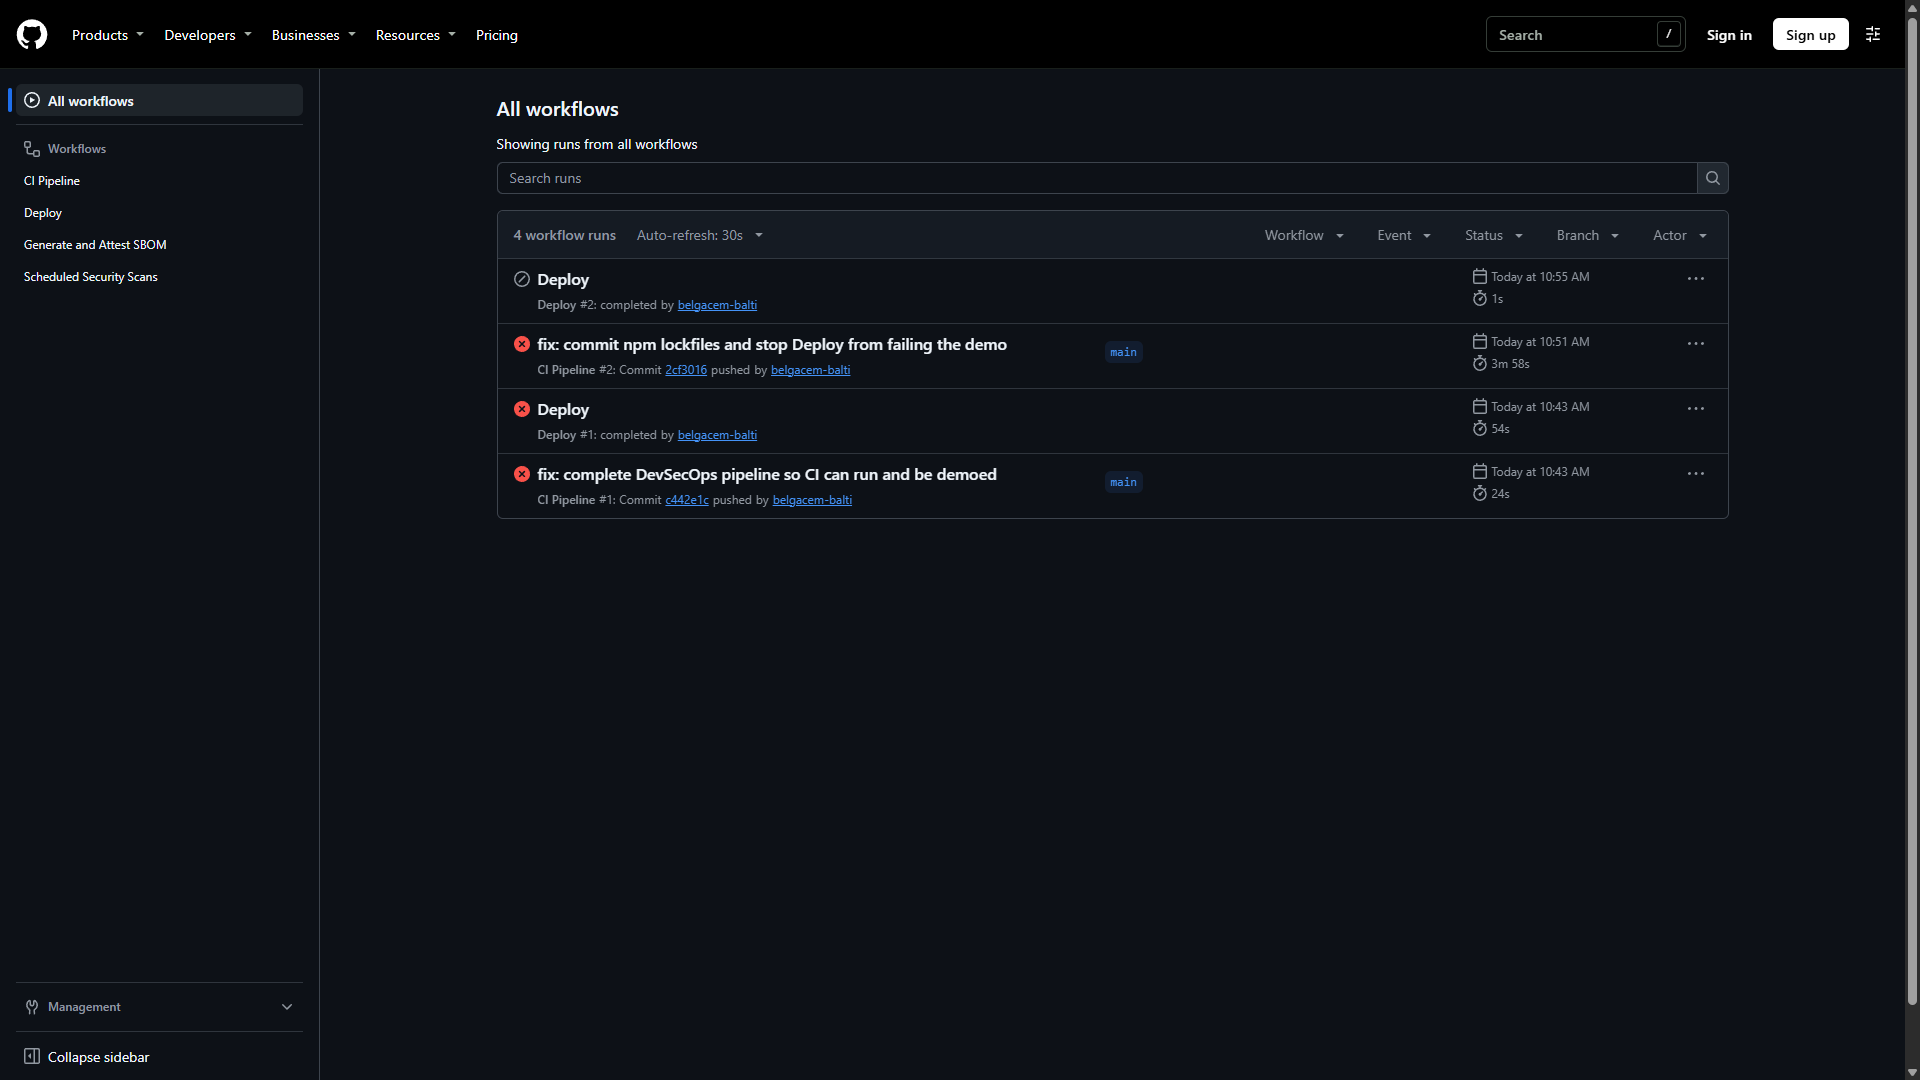
\includegraphics[width=0.95\textwidth]{figures/00-actions-all-runs.png}
\caption{GitHub Actions home (6 Nov 2026). Four runs: two CI Pipeline, two Deploy. Left sidebar lists the four workflow files.}
\end{figure}
\noindent\textbf{How to read Figure~\thefigure.}
The grey Deploy \#2 with a skipped icon is the desired control: deploy must not start when CI failed.
The two red CI rows are not the same failure: \#1 died in 24\,s (install), \#2 ran 3\,m\,58\,s (almost the full path).
The left column is the catalogue of controls: CI (every push), Deploy (after success), SBOM (on release), Scheduled Security Scans (ZAP + full Trivy, Monday or manual).

\begin{figure}[ht]
\centering
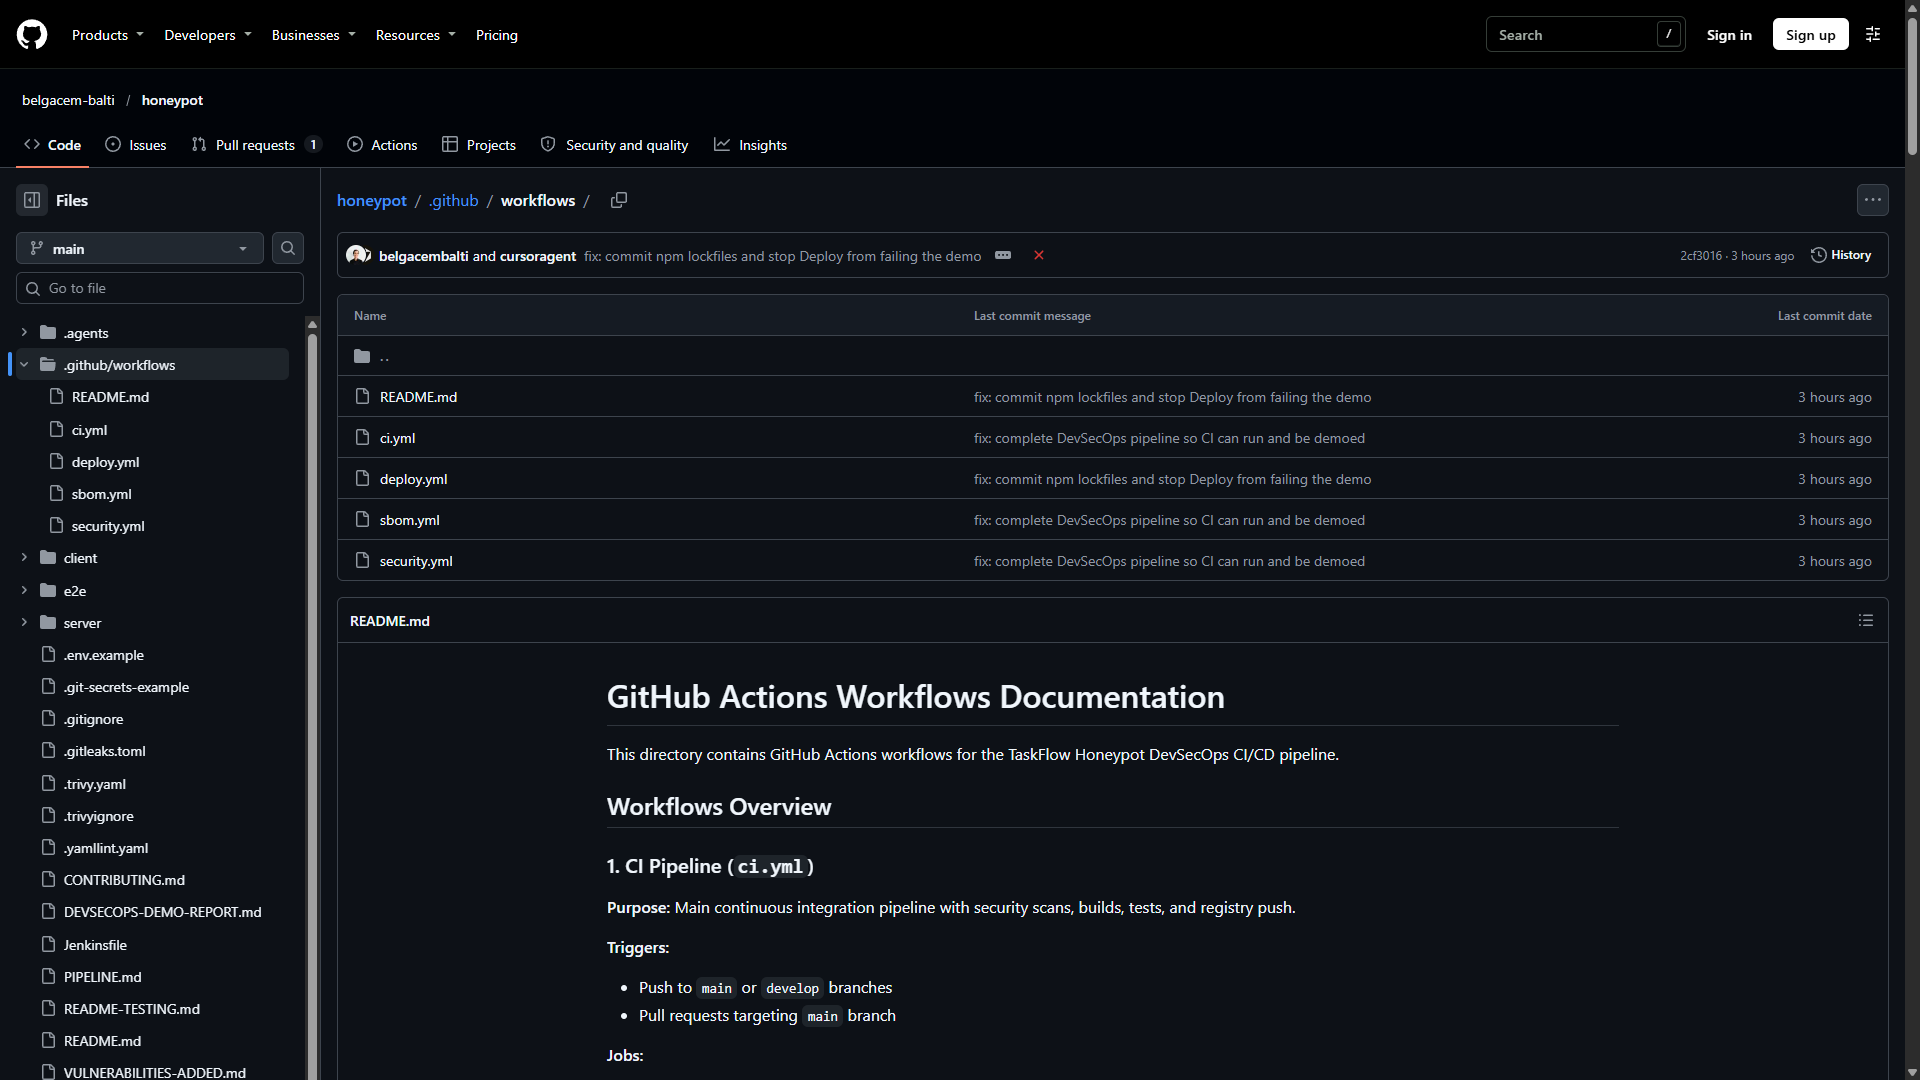
\includegraphics[width=0.95\textwidth]{figures/04-workflows-folder.png}
\caption{Repository view of \texttt{.github/workflows/}: \texttt{ci.yml}, \texttt{deploy.yml}, \texttt{sbom.yml}, \texttt{security.yml}, plus the operator README.}
\end{figure}
\noindent\textbf{How to read Figure~\thefigure.}
This is the ``source of truth'' for GitHub. Unlike a screenshot of a passing job, this figure shows the pipeline is versioned in git (Conventional Commits on the right).
A reviewer can open each YAML and match it to a tool in Section~4.

\begin{figure}[ht]
\centering
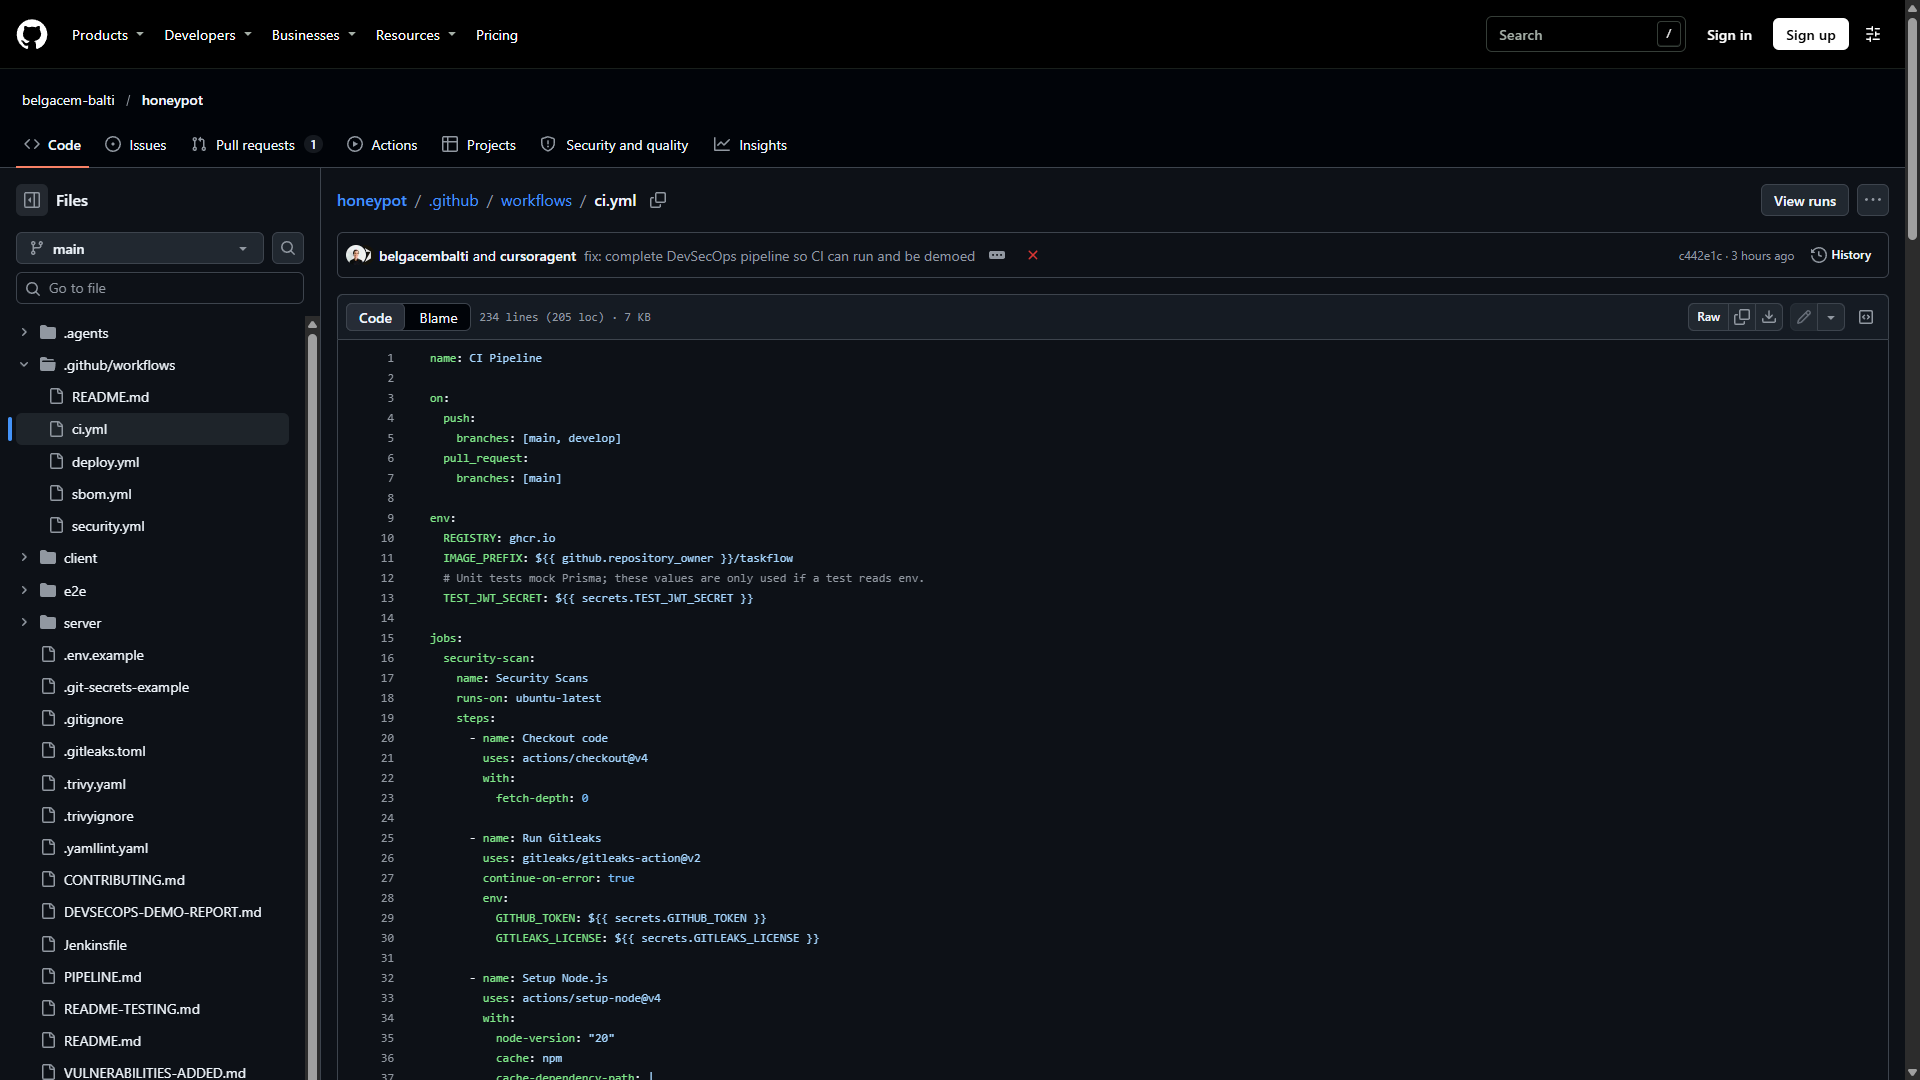
\includegraphics[width=0.95\textwidth]{figures/03-ci-yml-github.png}
\caption{Start of \texttt{ci.yml}: push/PR triggers, Gitleaks step with \texttt{continue-on-error}, Node 20 setup.}
\end{figure}
\noindent\textbf{How to read Figure~\thefigure.}
\texttt{fetch-depth: 0} matters: Gitleaks needs full git history, not a shallow clone.
\texttt{continue-on-error: true} on Gitleaks is the honeypot choice: planted secrets must not block the rest of the demo.
\texttt{cache: npm} with both lockfiles is why run \#1 exploded when the committed lockfile did not match \texttt{package.json}.

\begin{figure}[ht]
\centering
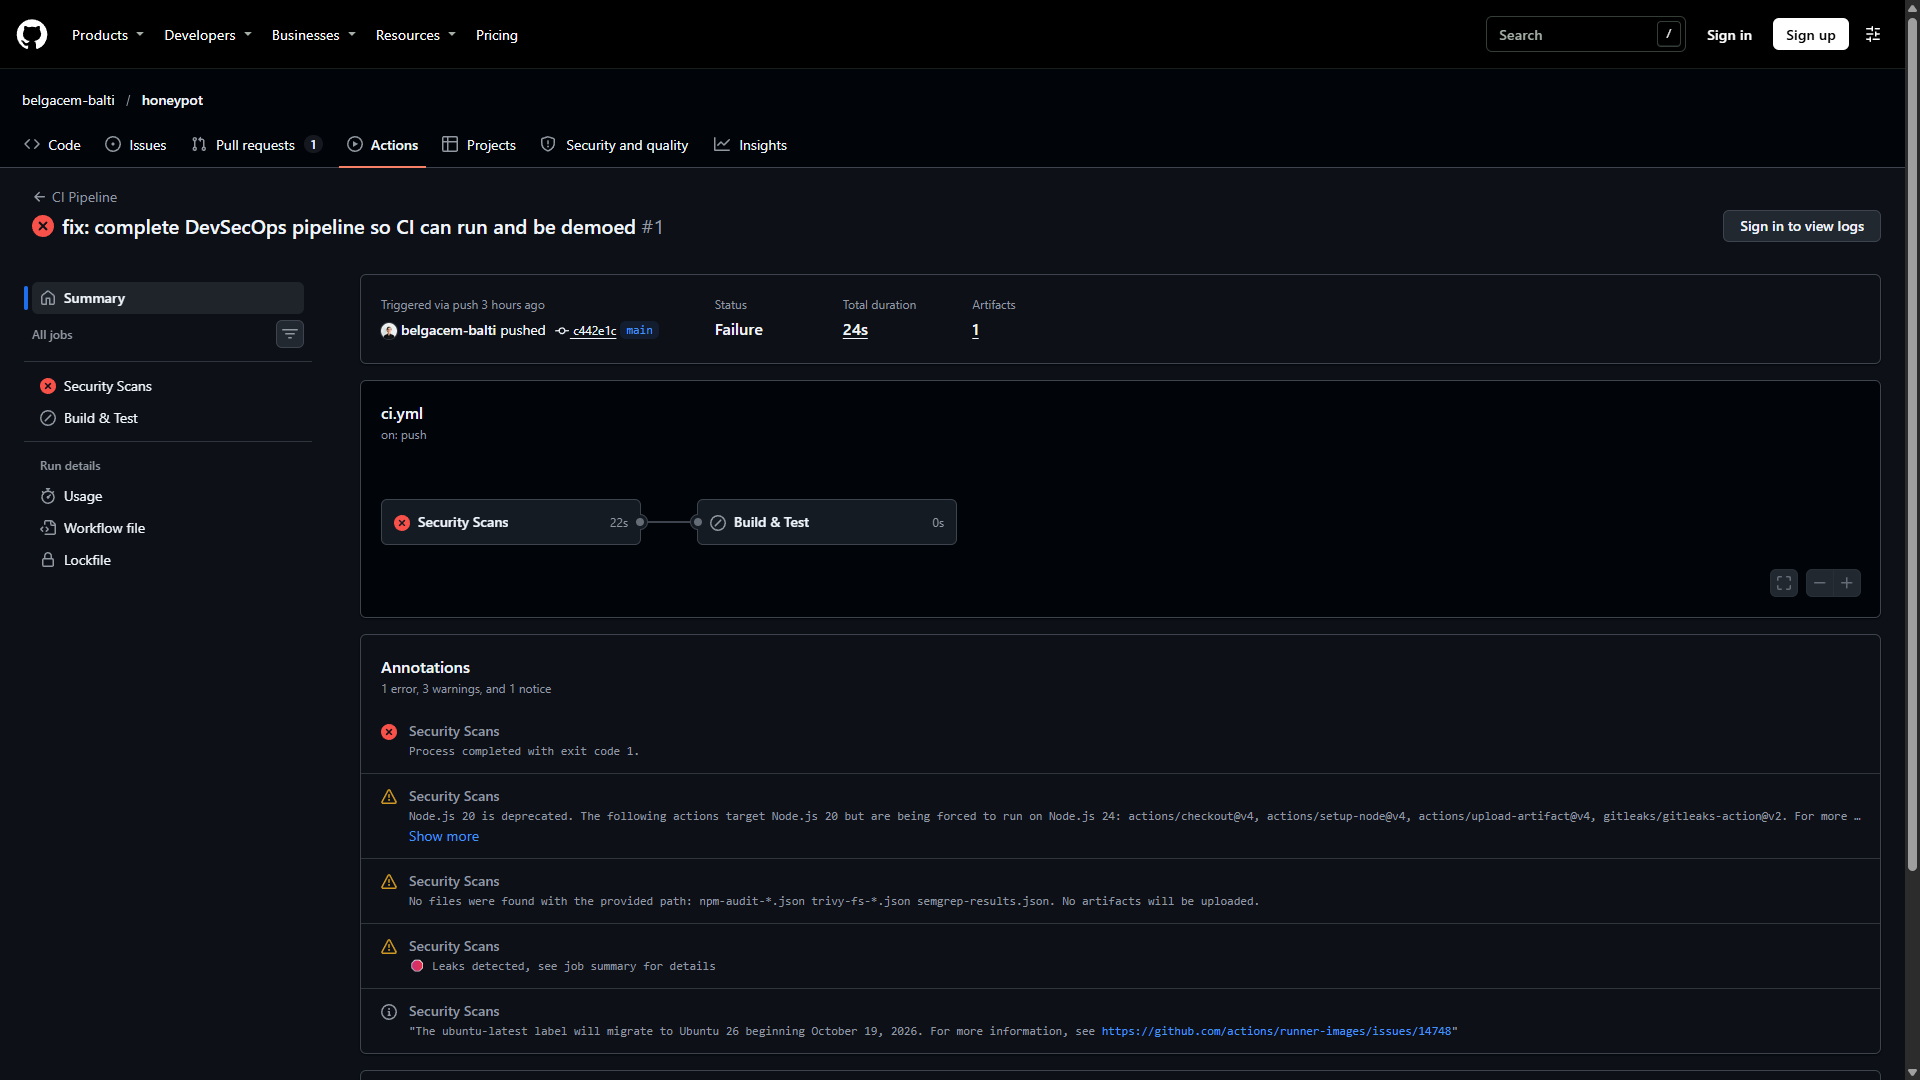
\includegraphics[width=0.95\textwidth]{figures/01-ci-run-lockfile-fail.png}
\caption{CI run \#1 (\texttt{c442e1c}). Graph: red Security Scans (22\,s) then grey Build \& Test (0\,s). Annotations include Gitleaks leaks and ``no artifacts''.}
\end{figure}
\noindent\textbf{How to read Figure~\thefigure.}
The \textbf{job graph} is the most important visual: Build never started because it \texttt{needs: security-scan}.
The pink annotation ``Leaks detected'' is Gitleaks doing its job on honeypot fixtures.
The yellow annotation ``No files were found \ldots npm-audit / trivy-fs'' means \texttt{npm ci} died before those files existed --- so this run cannot be used as evidence of Trivy or Semgrep.

\begin{figure}[ht]
\centering
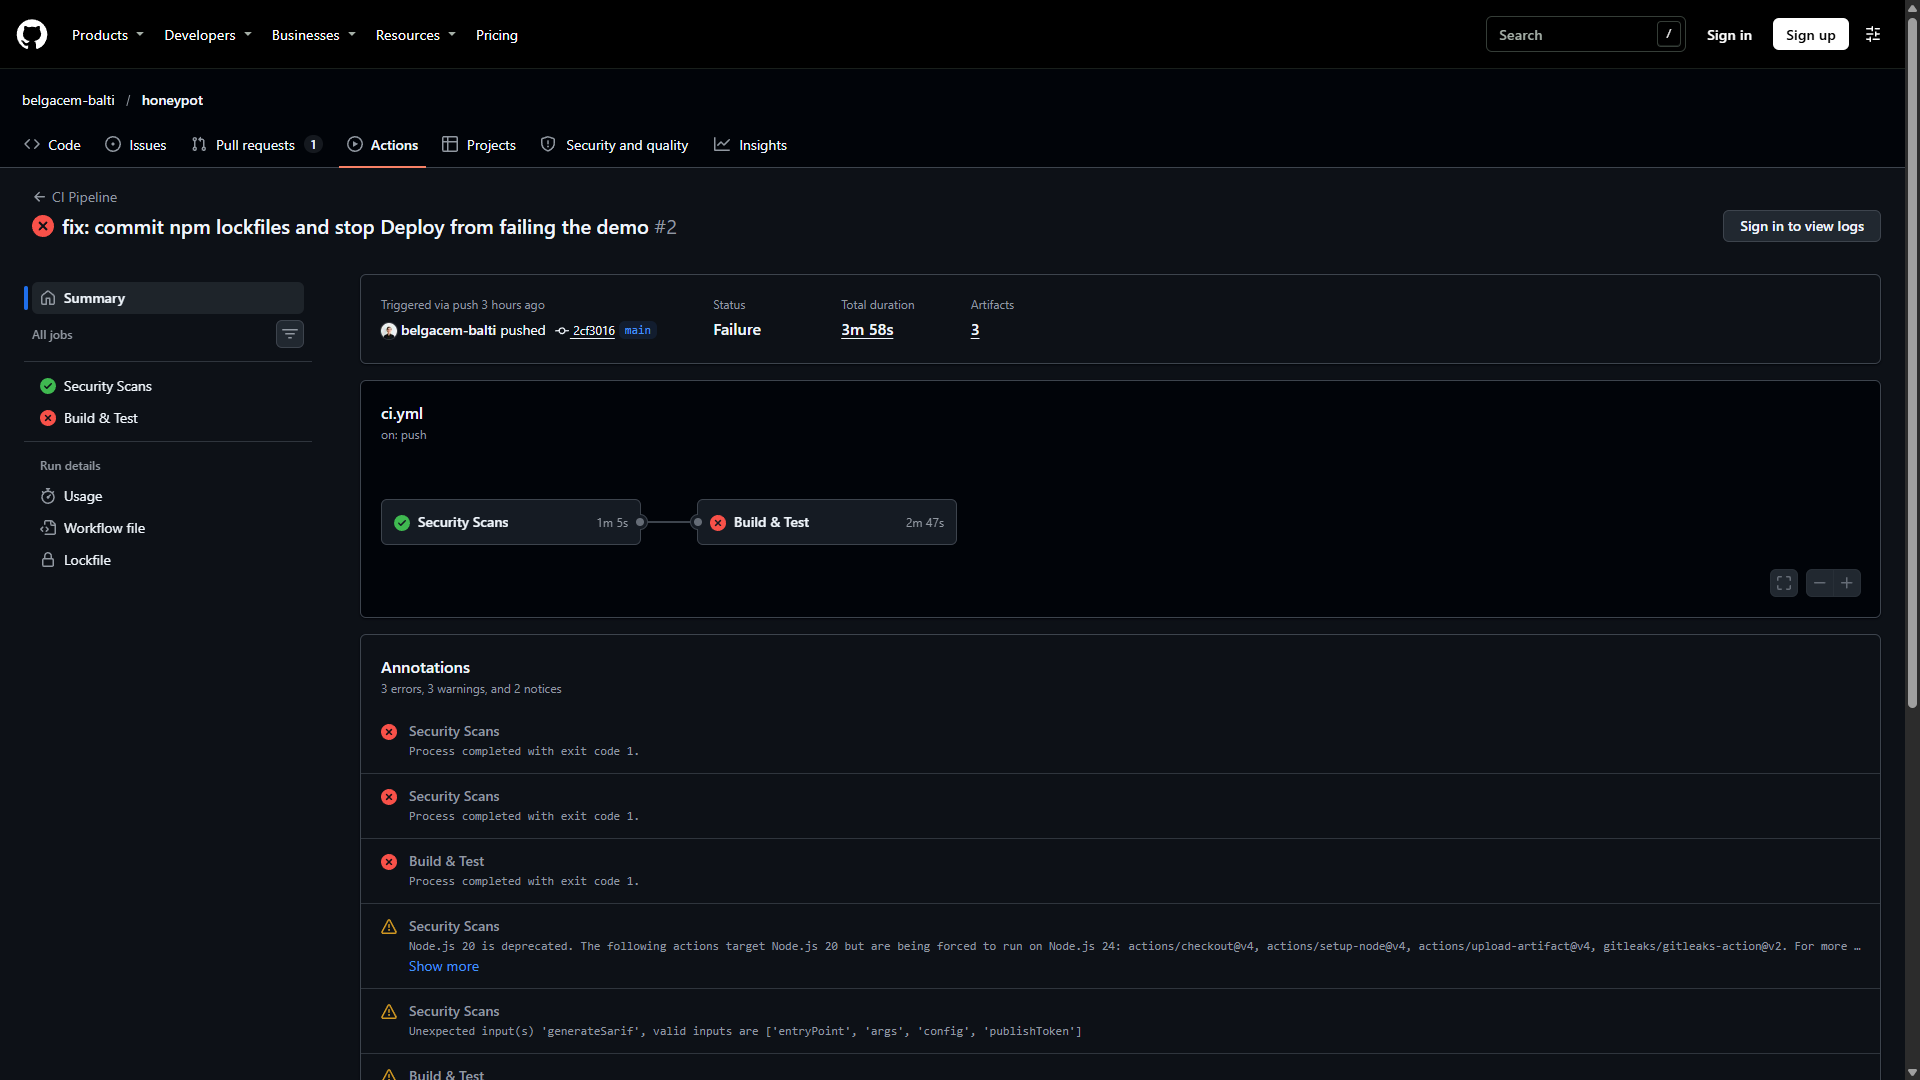
\includegraphics[width=0.95\textwidth]{figures/02-ci-run-after-lockfiles.png}
\caption{CI run \#2 (\texttt{2cf3016}). Green Security Scans (1\,m\,5\,s) feeding red Build \& Test (2\,m\,47\,s). Artifacts listed at the bottom of the run (not all visible here).}
\end{figure}
\noindent\textbf{How to read Figure~\thefigure.}
This is the run to cite for \textbf{Gitleaks, npm audit, Trivy fs, Semgrep, Jest, Vitest, Docker hardened build, Trivy image, SBOM}.
API job data shows those steps succeeded; the red X is only \texttt{Tag and push client image} (GHCR \texttt{packages: write}).
Duration jumped from 24\,s to $\approx$4\,min because the pipeline actually built two images and scanned them.

\subsection{Secret detection}

\begin{figure}[ht]
\centering
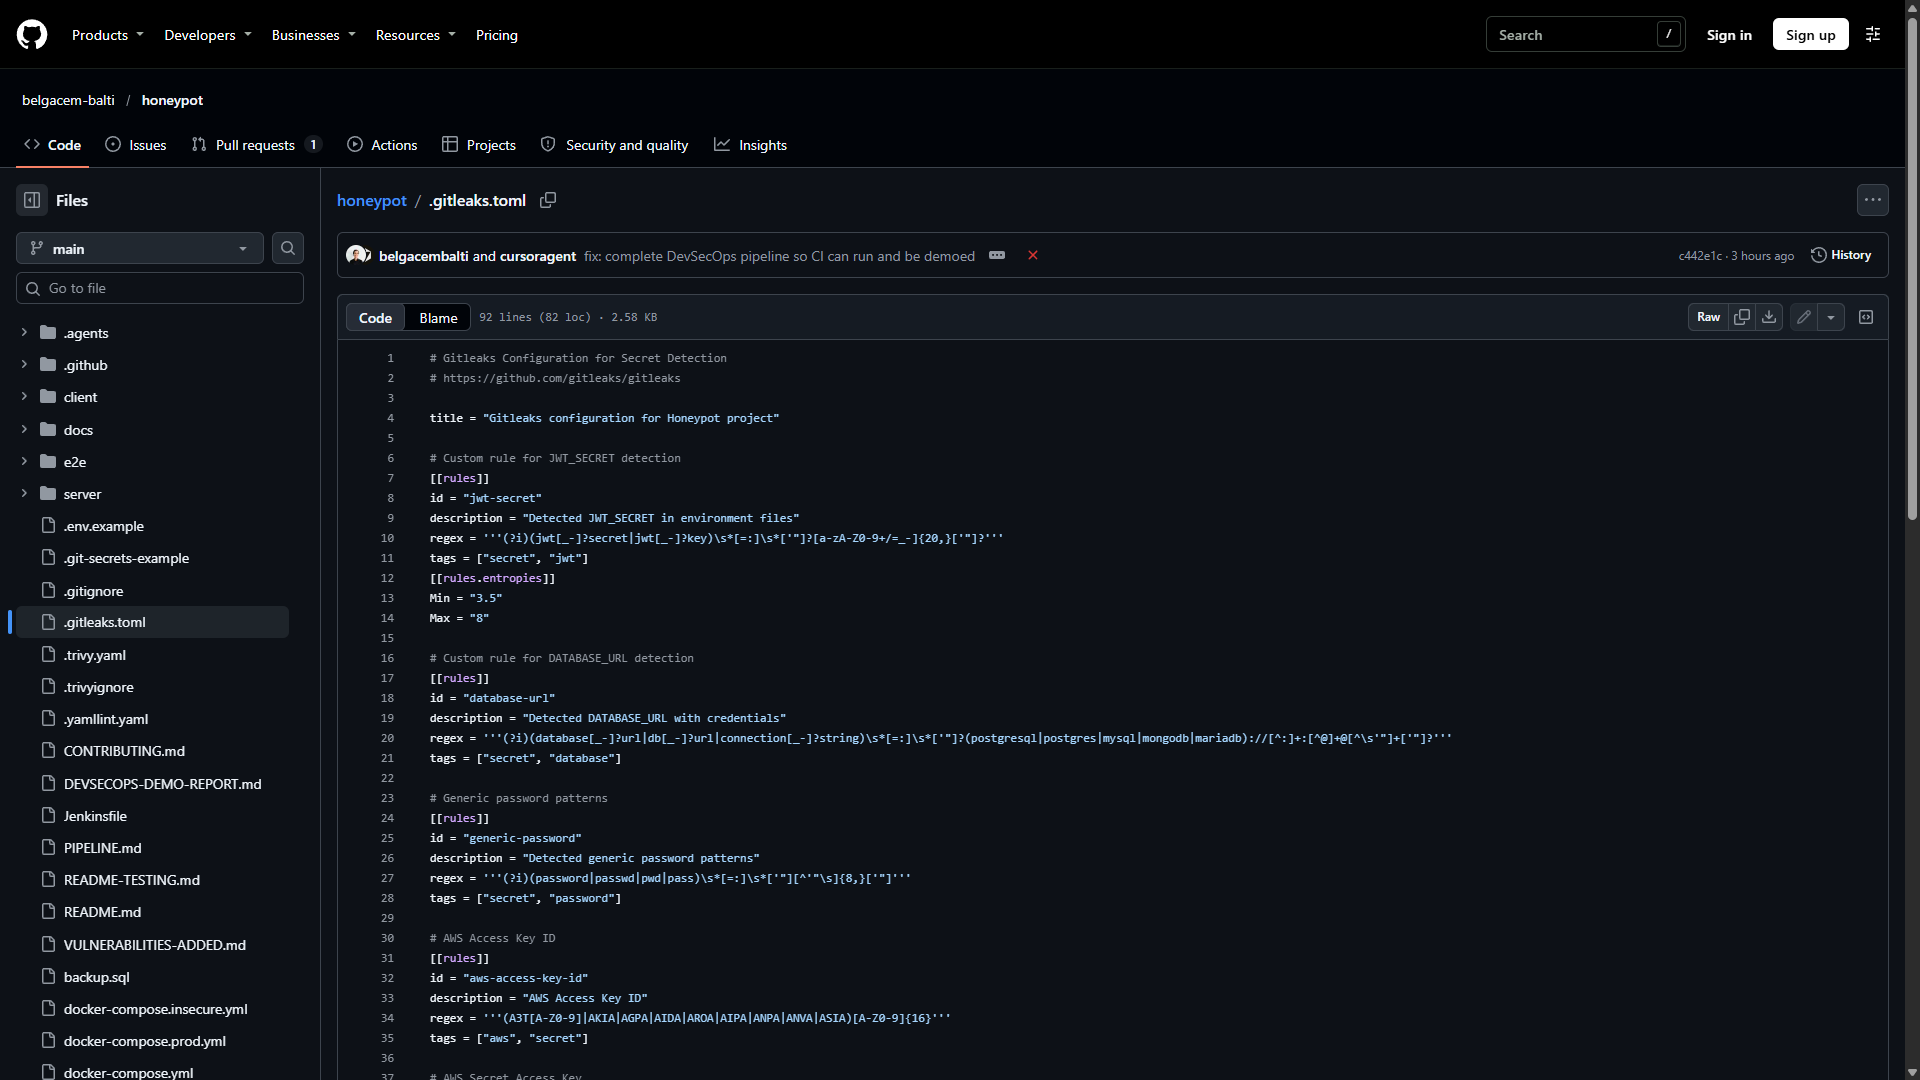
\includegraphics[width=0.95\textwidth]{figures/06-gitleaks-toml.png}
\caption{\texttt{.gitleaks.toml}: custom rules for \texttt{JWT\_SECRET}, \texttt{DATABASE\_URL}, generic passwords, and AWS access key IDs.}
\end{figure}
\noindent\textbf{How to read Figure~\thefigure.}
Rules are regexes, not a generic entropy-only scan. That is why this project catches \texttt{JWT\_SECRET=hardcoded-...} even when entropy is mediocre.
The allowlist (further down in the same file) skips \texttt{node\_modules} so CI uses git history instead of walking 100k vendor files.
Screenshot this file next to the Actions step \texttt{Run Gitleaks} once you are signed in.

\subsection{Hardened vs insecure runtime}

\begin{figure}[ht]
\centering
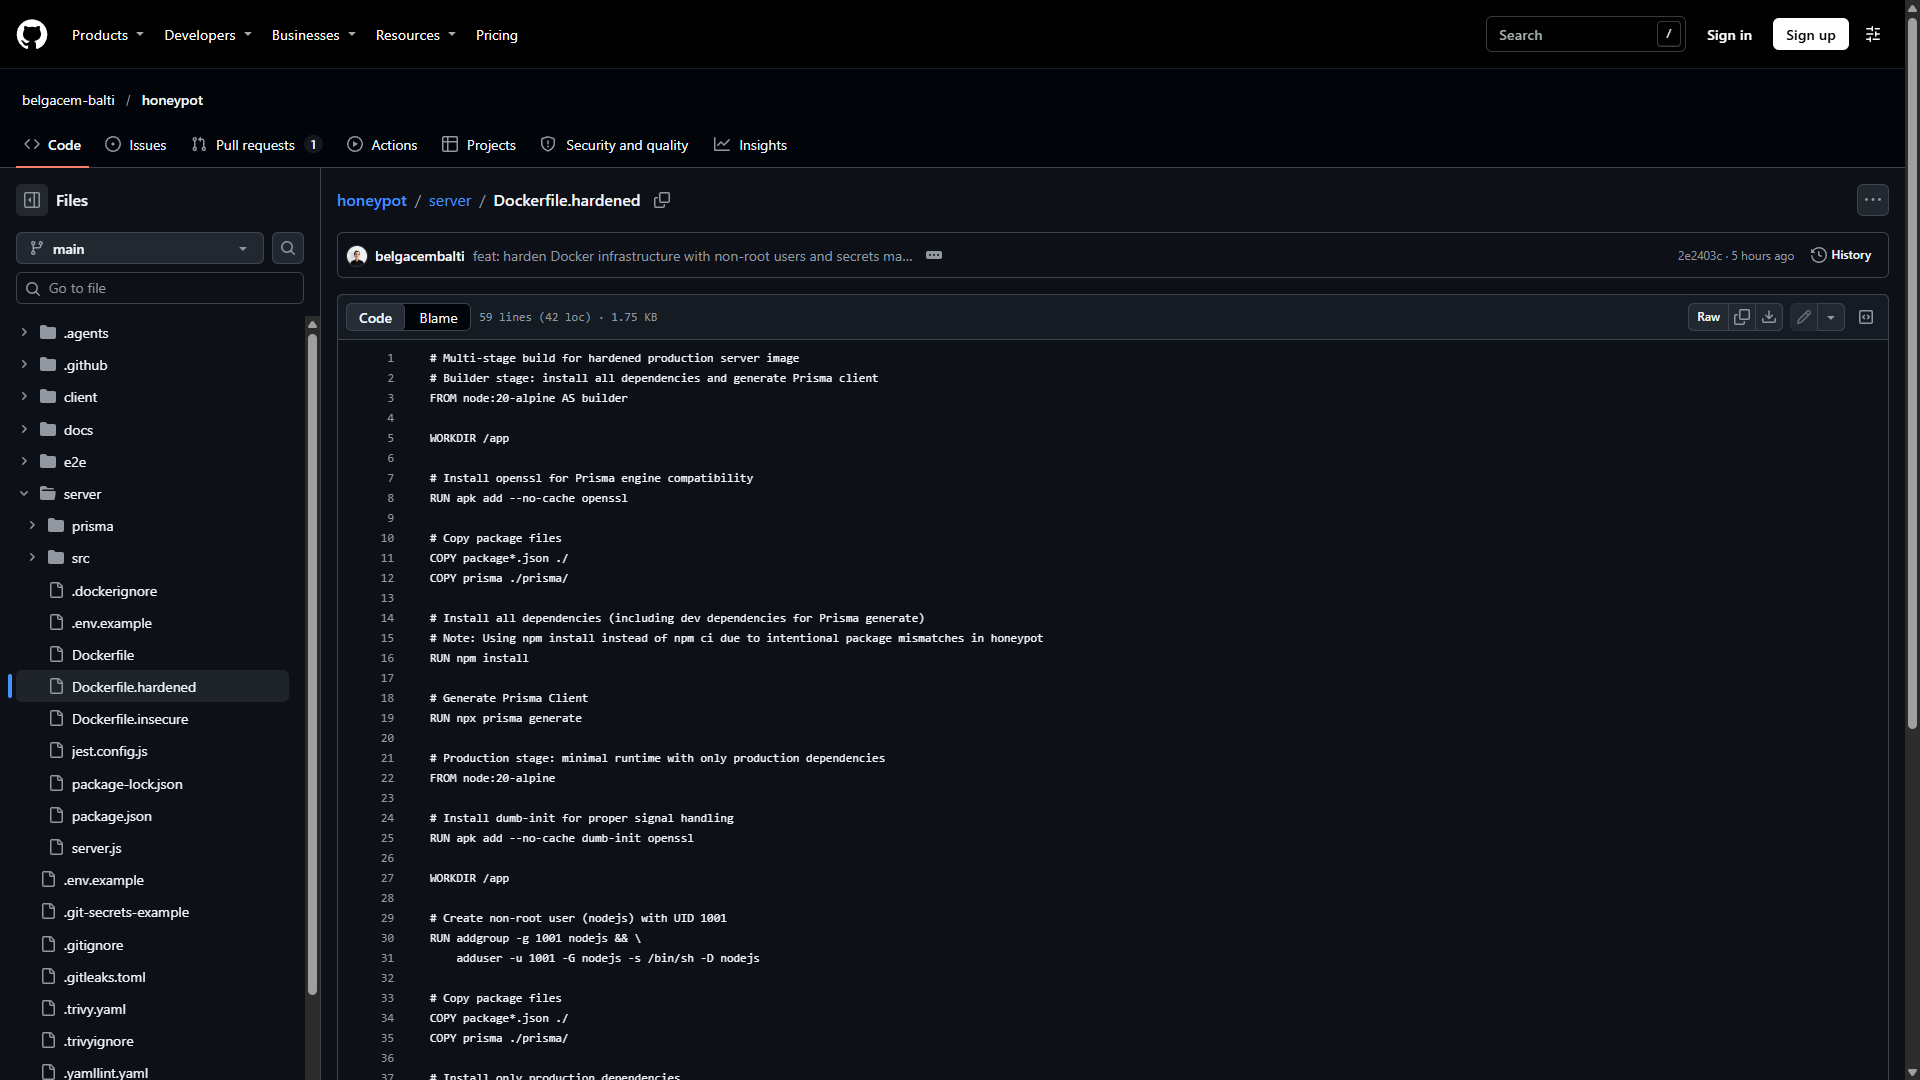
\includegraphics[width=0.95\textwidth]{figures/05-dockerfile-hardened.png}
\caption{\texttt{server/Dockerfile.hardened}: multi-stage \texttt{node:20-alpine}, Prisma generate in builder, non-root UID 1001.}
\end{figure}
\noindent\textbf{How to read Figure~\thefigure.}
Two \texttt{FROM} lines = two stages. The production stage never runs \texttt{npx prisma db push} (migrations stay operational, not in \texttt{CMD}).
\texttt{adduser -u 1001} is the countermeasure to ``container as root''.
CI \texttt{docker/build-push-action} points at this file, not at \texttt{Dockerfile} / \texttt{Dockerfile.insecure}.
Trivy image scan then inspects \emph{this} artifact.

\begin{figure}[ht]
\centering
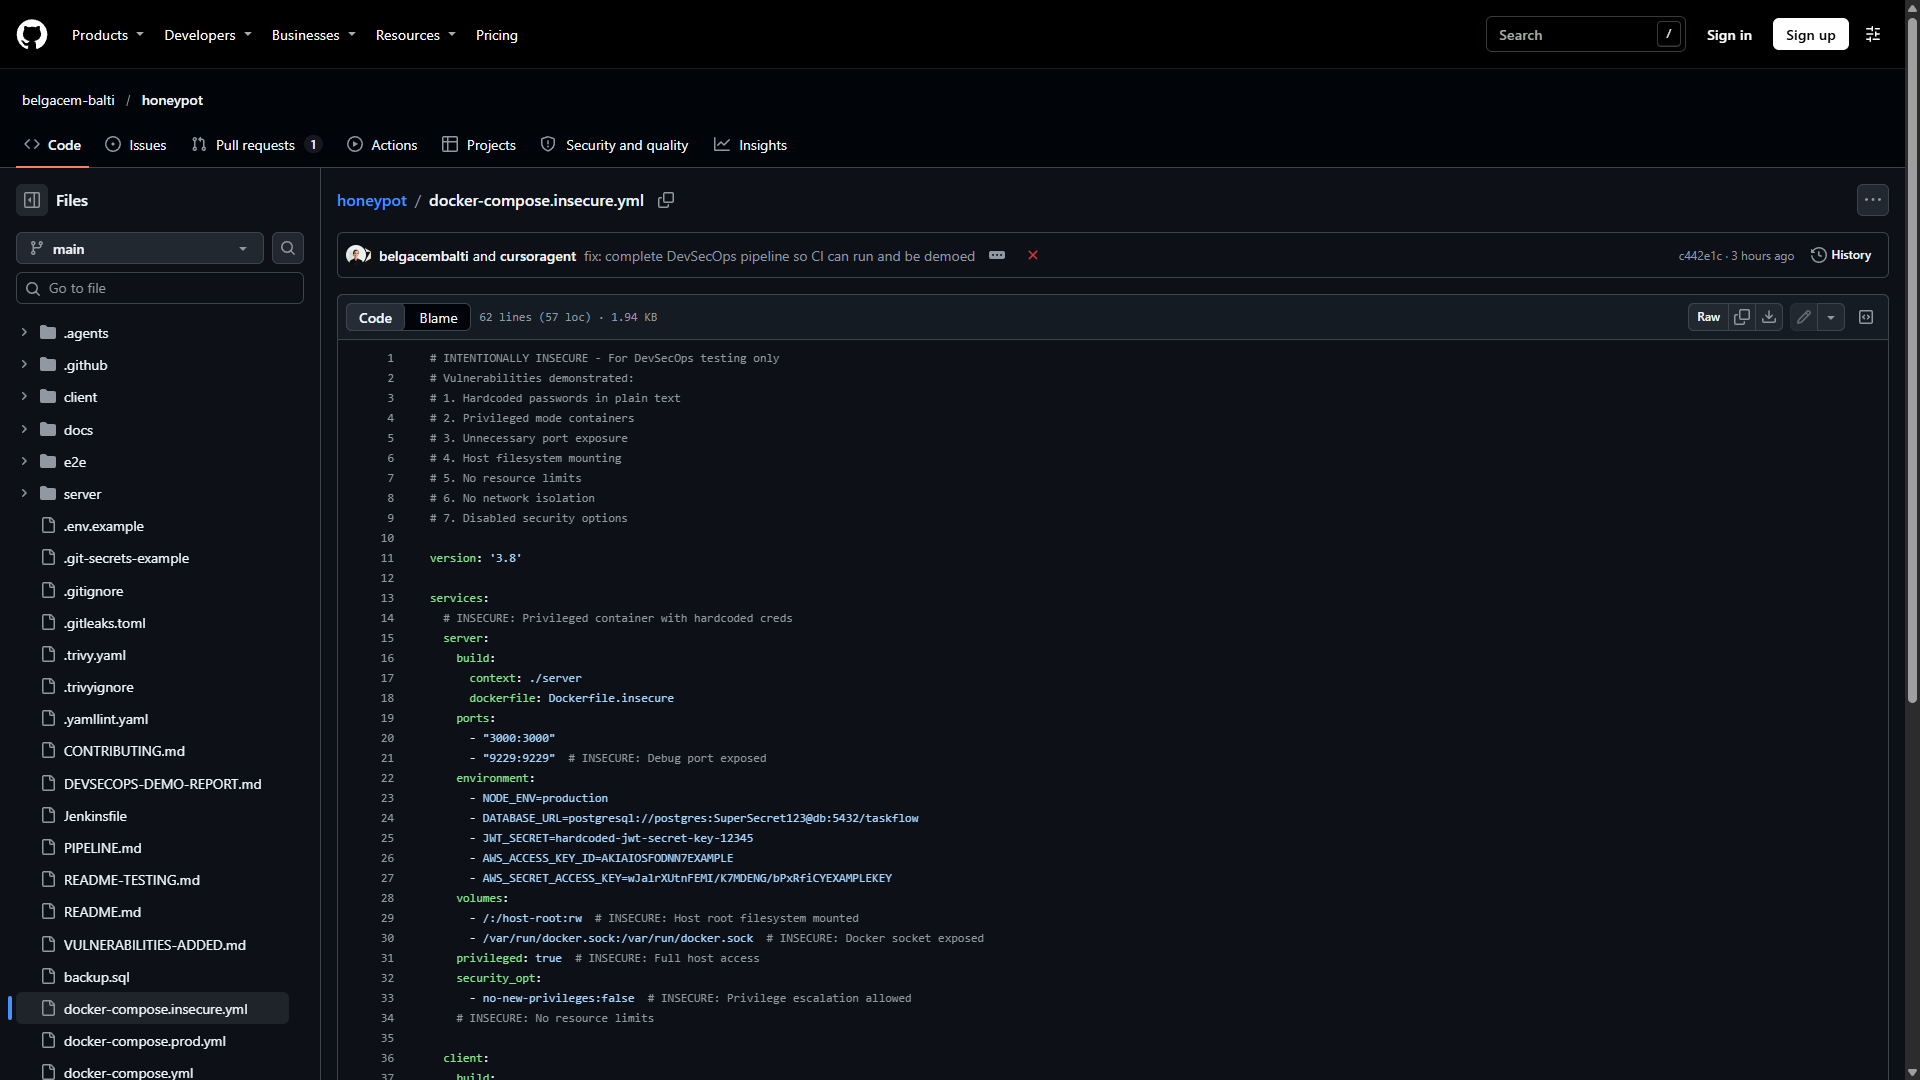
\includegraphics[width=0.95\textwidth]{figures/08-compose-insecure.png}
\caption{Honeypot bait: \texttt{docker-compose.insecure.yml} with hardcoded DB/JWT/AWS secrets, host root mount, Docker socket, \texttt{privileged: true}.}
\end{figure}
\noindent\textbf{How to read Figure~\thefigure.}
This file is the \textbf{before} state for containers. Privileged + \texttt{/var/run/docker.sock} is a trivial breakout.
Gitleaks and Trivy config scanning are expected to fire here.
It is \emph{not} what Deploy uses; it exists so the report can show a bad baseline.

\begin{figure}[ht]
\centering
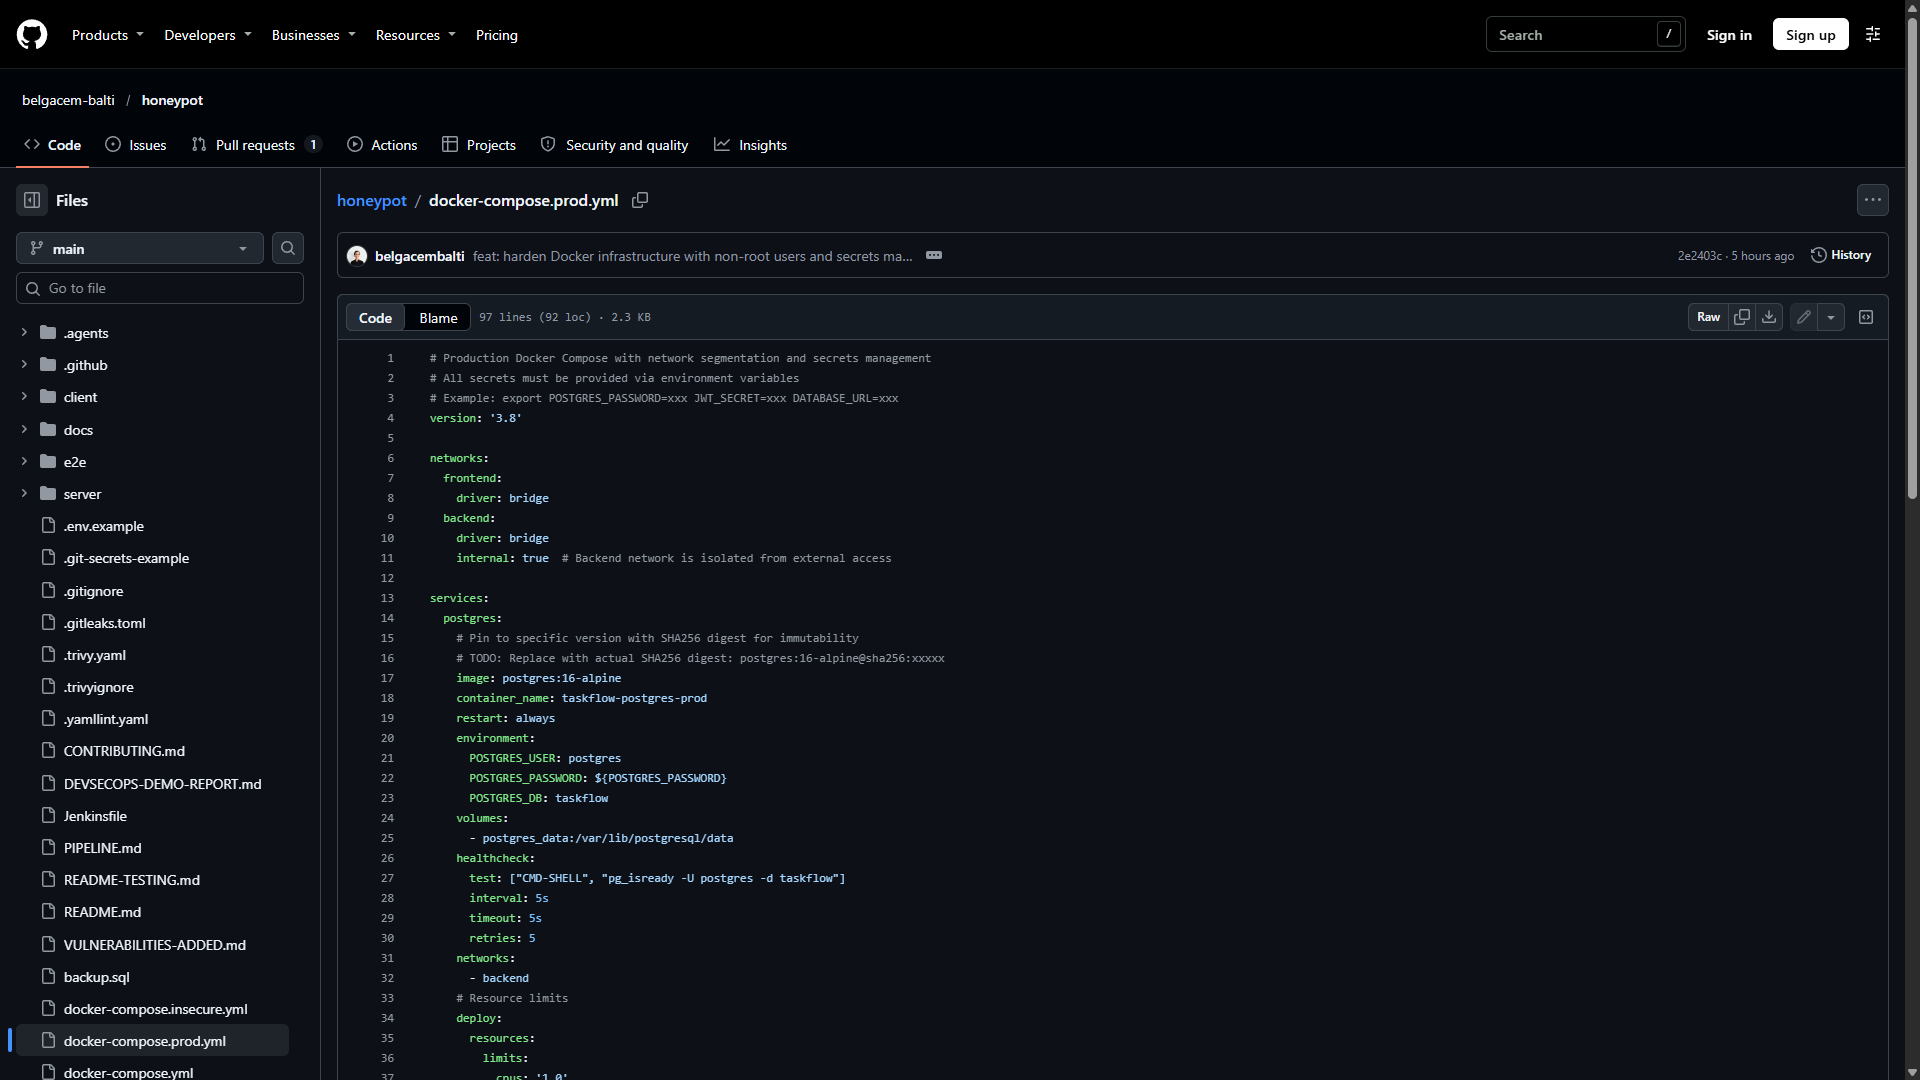
\includegraphics[width=0.95\textwidth]{figures/07-compose-prod.png}
\caption{\texttt{docker-compose.prod.yml}: \texttt{frontend}/\texttt{backend} networks, \texttt{backend} marked \texttt{internal: true}, \texttt{POSTGRES\_PASSWORD: \$\{POSTGRES\_PASSWORD\}}.}
\end{figure}
\noindent\textbf{How to read Figure~\thefigure.}
\texttt{internal: true} on \texttt{backend} means Postgres is not reachable from the internet --- only from services on that network (the API).
No password literals: if the GitHub secret is missing, Compose must fail or skip (Deploy \#1 vs \#2).
Resource \texttt{deploy.resources.limits} (CPU/memory) appear just below the crop; they cap noisy-neighbour DoS.

\begin{figure}[ht]
\centering
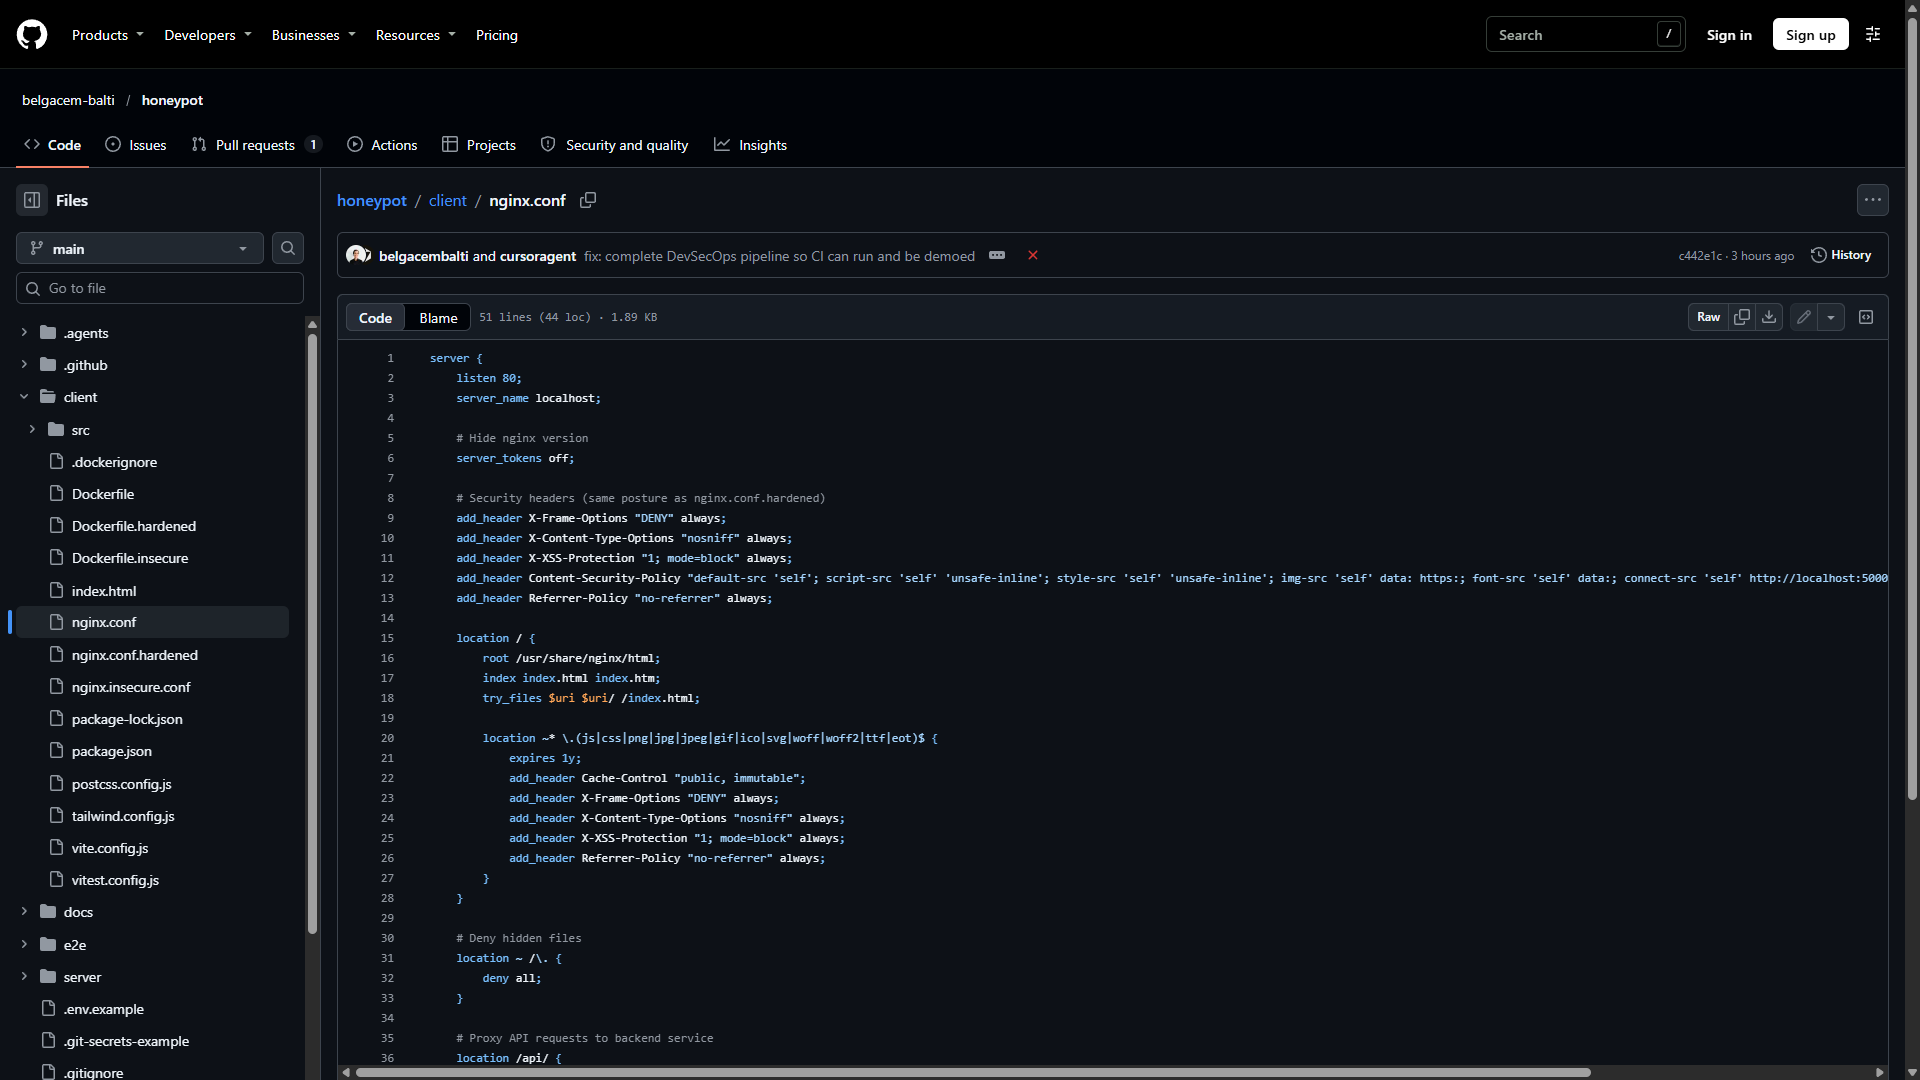
\includegraphics[width=0.95\textwidth]{figures/09-nginx-headers.png}
\caption{\texttt{client/nginx.conf}: \texttt{server\_tokens off}, CSP, \texttt{X-Frame-Options DENY}, \texttt{nosniff}, deny hidden files, \texttt{/api/} proxy.}
\end{figure}
\noindent\textbf{How to read Figure~\thefigure.}
Headers are the countermeasure to clickjacking (frame), XSS (CSP), MIME sniffing (\texttt{nosniff}).
They are repeated inside the static-asset location because nginx nested \texttt{add\_header} replaces parent headers instead of merging them.
ZAP (next figure) is the runtime proof that those headers exist on the wire, not only in git.

\subsection{DAST and Jenkins}

\begin{figure}[ht]
\centering
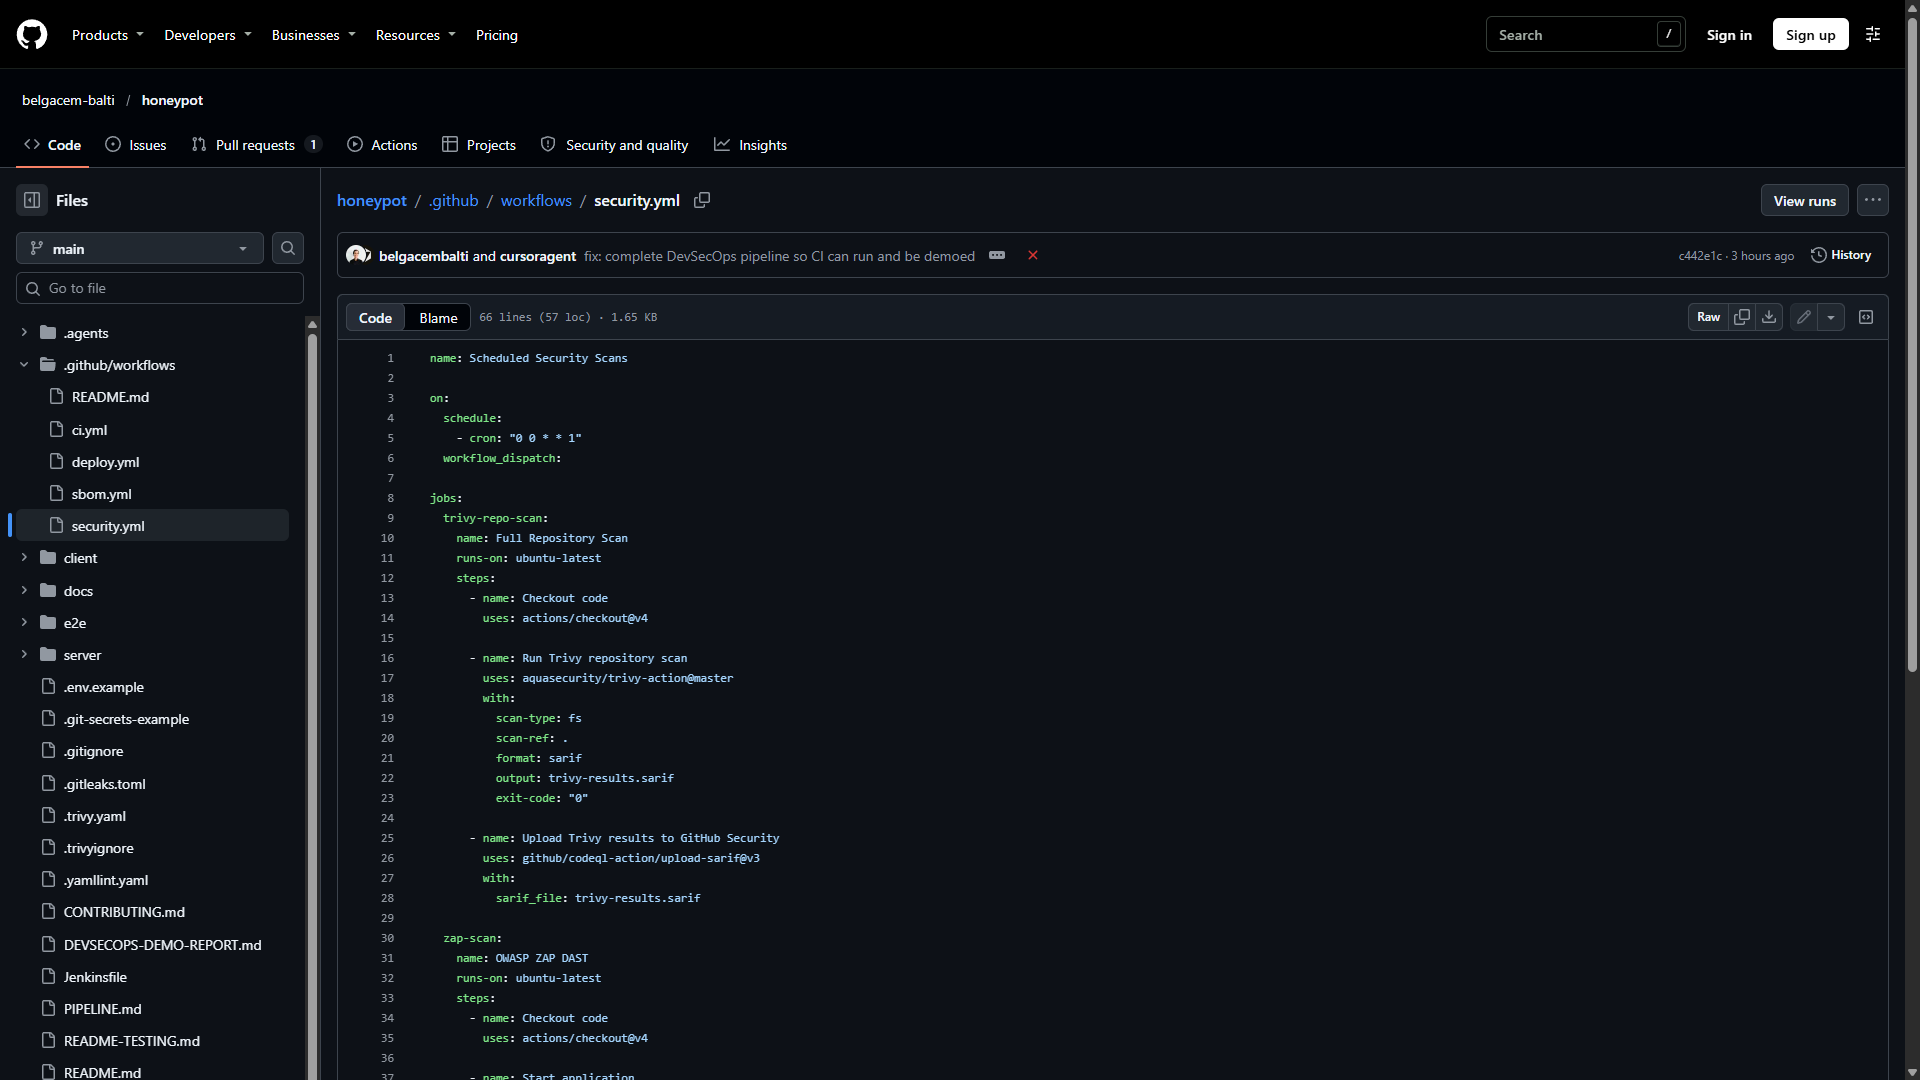
\includegraphics[width=0.95\textwidth]{figures/10-security-yml-zap.png}
\caption{\texttt{security.yml}: weekly cron plus \texttt{workflow\_dispatch}; Trivy SARIF upload; job \texttt{zap-scan} (OWASP ZAP DAST) starts below the crop.}
\end{figure}
\noindent\textbf{How to read Figure~\thefigure.}
ZAP is \textbf{not} in \texttt{ci.yml}. To screenshot it: Actions $\rightarrow$ Scheduled Security Scans $\rightarrow$ Run workflow.
The Trivy job writes SARIF into the GitHub Security tab (\texttt{upload-sarif@v3}).
\texttt{exit-code: "0"} again: findings are evidence, not a red weekly email for the honeypot.

\begin{figure}[ht]
\centering
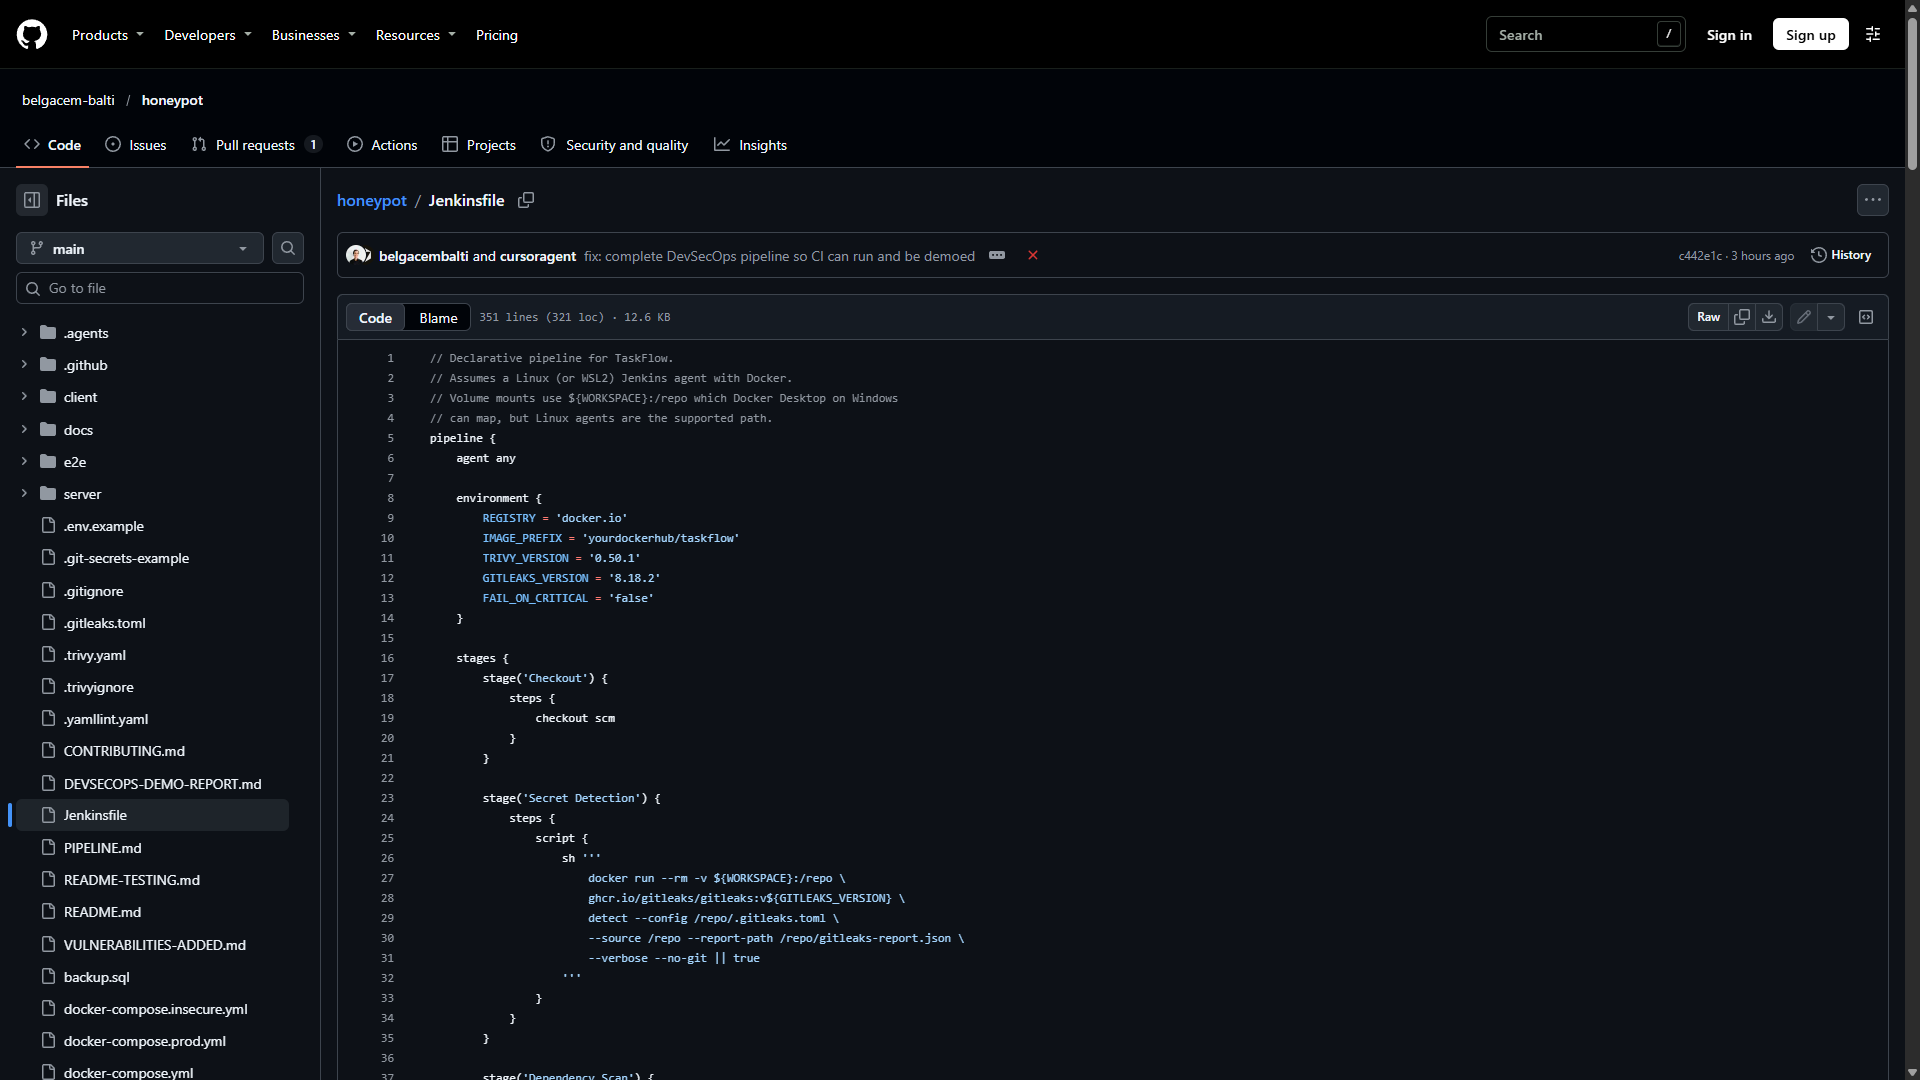
\includegraphics[width=0.95\textwidth]{figures/11-jenkinsfile.png}
\caption{Jenkinsfile: Linux agent, pinned Trivy 0.50.1 and Gitleaks 8.18.2, \texttt{FAIL\_ON\_CRITICAL=false}, Checkout then Secret Detection via \texttt{docker run}.}
\end{figure}
\noindent\textbf{How to read Figure~\thefigure.}
Same tools as GitHub Actions, different runner. \texttt{\$\{WORKSPACE\}:/repo} is the Linux volume form.
\texttt{|| true} after Gitleaks matches \texttt{continue-on-error} in Actions.
This figure answers ``is the pipeline locked to GitHub?'' --- no.

\section{Where to click for tool logs}

Sign in (anonymous GitHub hides logs). Open CI run \#2. Expand the job, then the step. Capture the step title + log.

\begin{tcolorbox}[common, tabularx={Y Y Y}]
\textbf{Tool} & \textbf{Job} & \textbf{Step name in the UI} \\
Gitleaks & Security Scans & \texttt{Run Gitleaks} \\
npm audit & Security Scans & \texttt{Run npm audit (client/server)} \\
Trivy fs & Security Scans & \texttt{Run Trivy filesystem scan (...)} \\
Semgrep & Security Scans & \texttt{Run Semgrep} \\
Jest / Vitest & Build \& Test & \texttt{Run server tests} / \texttt{Run client tests} \\
Trivy image & Build \& Test & \texttt{Scan client/server image with Trivy} \\
SBOM & Build \& Test & \texttt{Generate SBOM for client/server} \\
ZAP & OWASP ZAP DAST (other workflow) & \texttt{Run ZAP baseline scan}
\end{tcolorbox}

On the run \textbf{Summary}, download artifacts \texttt{security-scan-results} and \texttt{image-scan-results} and screenshot the JSON in an editor (second evidence per tool).

\section{Recommendations}

\begin{enumerate}[leftmargin=1.2em,itemsep=3pt]
  \item Keep \texttt{permissions.packages: write} so the GHCR push in Build \& Test can succeed; re-run CI and screenshot a green graph if possible.
  \item Sign in and capture the eight tool steps above; anonymous screenshots only show the job graph.
  \item For a real product: Trivy \texttt{exit-code: 1} and Jenkins \texttt{FAIL\_ON\_CRITICAL=true}.
  \item Store \texttt{JWT\_SECRET}, \texttt{DATABASE\_URL}, \texttt{POSTGRES\_PASSWORD} in GitHub Environments with reviewers on production.
  \item Trigger \textbf{Scheduled Security Scans} once to obtain ZAP HTML (\texttt{zap-report.html}).
  \item Do not treat a green honeypot pipeline as production-safe: pins and \texttt{vulnerable.js} are still in the tree.
\end{enumerate}

\vspace{0.8em}
{\color{muted}\small Repository: \url{https://github.com/belgacem-balti/honeypot} \quad Date: 6 November 2026.}

\end{document}
